\section{Program}
As said previously, the code that was provided to us is a parallel code. The master splits the data and send each part to a slave, that computes the clusters and send the result back to the master. Then the master gathers these results.

There are several ways for the slaves to compute the clusters. One of these methods was already implemented in the code: the Spectral clustering. Then we implemented two new methods: the Mean shift and the Kernel k-means. The method is chosen in the parameter file.
\begin{center}
\begin{figure}[h!]
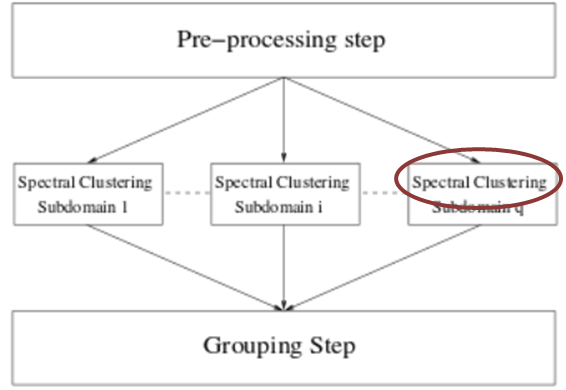
\includegraphics[width=0.3\textwidth, height=5.5cm]{Image/parallel2.png}
\caption{Structure of the parallel program}
\end{figure}
\end{center}

The aim is to split the data points into clusters, the points in the same clusters being as similar as possible. The similarity can depend on the distance for example, or on the color. Here is an example of clustering based on distance.
\begin{center}
\begin{figure}[h!]
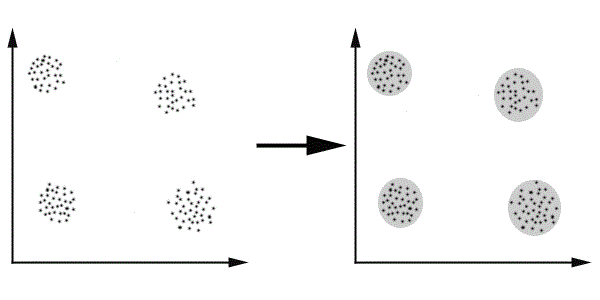
\includegraphics[width=0.3\textwidth, height=5.5cm]{Image/clust.png}
\caption{Example of clustering based on distance}
\end{figure}
\end{center}
